\section{Autorisierung}

\subsection{Benutzerrollen}

Die Rolle eines Benutzers wird im User-Model in Form eines \emph{ActiveRecord::Enum} abgebildet. Hier wird bewusst ein Sting-Wert in der Datenbank
bevorzugt, da sich ein Integer-Wert beim Hinzufügen von neuen Rollen verändern könnte. Ausserdem ist so in der Datenbank die Benutzerrolle immer
direkt ersichtlich. Auf den Enum wird auch der Default-Wert \enquote{candidate} gesetzt, sodass neue Benutzer, die eingeladen werden, automatisch dieser Rolle zugeteilt werden. 

\begin{codebox}
\begin{minted}{ruby}
class User < ApplicationRecord
  enum :role, { admin: 'admin', candidate: 'candidate' }, default: :candidate
end
\end{minted}
\end{codebox}

Die Benutzerrolle kann dann auf jeder User-Instanz folgendermassen abgerufen werden:

\begin{figure}[H]
  \centering
  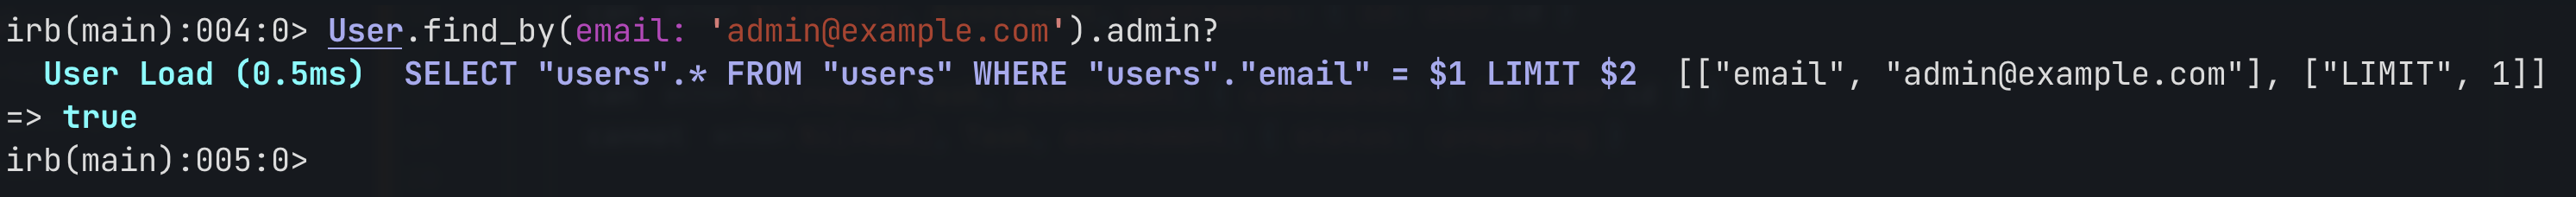
\includegraphics[width=\textwidth]{images/enum.png}
\end{figure}

\subsection{CanCanCan}

Als Autorisierungssystem wird, wie in \ref{sec:authorization} entschieden wurde, das \enquote{CanCanCan} Gem eingesetzt.
Dieses generiert nach der Installation eine Konfigurationsdatei \emph{app/models/abilities.rb}, in der
den Benutzern, basierend auf deren Rollen, sogenannte \enquote{Abilities} zugeteilt werden können.

Eine Ability-Definition kann grundsätzlich in drei Teile aufgeteilt werden und sagt gewissermassen aus: 
\emph{was darf ich?}, \emph{auf welcher Ressource darf ich?} und \emph{unter welchen Bedingungen darf ich?}

\begin{codebox}
\begin{minted}{ruby}
def candidate_abilities(user)
  can :index, Assessment, candidates: { id: user.id }

  can :read, Task, assessment: { candidates: { id: user.id } }
  cannot :read, Task, assessment: { status: :preparing }

  can :create, Solution, task: { assessment: { status: :open } }
  can :read, Solution, user_id: user.id
  can :update, Solution, user_id: user.id, task: { assessment: { status: :open } }

  can :read, Comment, solution: { user_id: user.id }
end
\end{minted}
\end{codebox}

Ein \mintinline{ruby}{:candidate} kann dementsprechend:
\begin{itemize}
  \item Nur die Assessments sehen, zu denen dieser auch Eingeladen wurde
  \item Tasks ansehen, allerdings erst, wenn das Assessment durch einen Admin gestartet wurde
  \item Lösungen erstellen, einsehen und bearbeiten, jedoch nur die eigenen
  \item Korrektur-Kommentare zu dem abgegebenen Lösungen sehen
\end{itemize}

\newpage

Ein Benutzer mit der Rolle \mintinline{ruby}{:admin} ist zu fast allem berechtigt, jedoch kann dieser:
\begin{itemize}
  \item Keine Lösungen erstellen oder bearbeiten
  \item Das Assessment und die Aufgaben nicht editieren, wenn dieses bereits gestartet wurde
\end{itemize}

\begin{codebox}
\begin{minted}{ruby}
def admin_abilities(_user)
  can :manage, :all

  cannot :edit, Assessment, status: %i[open reviewing closed]
  cannot %i[create update destroy], Task, assessment: { status: %i[open reviewing closed] }
  cannot %i[create update], Solution
end
\end{minted}
\end{codebox}
  
Die mitgelieferten Controller-Helper \mintinline{ruby}{load_resource} und \mintinline{ruby}{authorize_resource} erleichtern 
das Autorisieren der einzelnen Ressourcen und wurden daher in allen Controller-Klassen eingesetzt. Dadurch ist auch ein Grossteil vom \gls{boilerplate} Code
in den Controllern weggefallen.

Die Helper agieren wie eine \mintinline{ruby}{before_action} und werden daher vor jeder Action in den Controllern ausgeführt.
Grundsätzlich machen sie Folgendes:

\begin{enumerate}
  \item Autorisieren und laden nur die Objekte, die der Benutzer auch sehen darf
  \item Setzten automatisch die entsprechenden Instanzvariablen
\end{enumerate}

Es können auch, dem Routing entsprechend, mehrere Ressourcen geladen werden:
\begin{codebox}
\begin{minted}{ruby}
class TasksController < ApplicationController
  load_and_authorize_resource :assessment
  load_and_authorize_resource through: :assessment
  ...
end
\end{minted}
\end{codebox}

In den Views werden dann den Berechtigungen entsprechend einzelne Bedienelemente ein- oder ausgeblendet.
So wird beispielsweise auf der Assessment-Index Seite der Create-Button für Bewerber ausgeblendet, da diese keines
erstellen können:

\begin{codebox}
\begin{minted}{ruby}
- if can?(:create, Assessment)
  = link_to new_assessment_path(@assessment), class: 'btn btn-primary' do
    i.bi-plus-lg.me-2
    = t('buttons.crud.assessment.create')
\end{minted}
\end{codebox}

Durch CanCanCan konnten viele Views wiederverwendet werden und es mussten keine Extra-Seiten für die verschiedenen Rollen
erstellt werden. So werden beispielsweise auf der Seite, auf der das Assessment gelöst wird, alle
\emph{Solutions} über die entsprechende Instanzvariable gerendert. 

So sieht zwar jeder Benutzer nur seine eigene Lösung, der Admin hingegen kann alle sehen. 
So kann dieselbe Seite für das Lösen und Korrigieren eines Assessments verwendet werden.

\begin{codebox}
\begin{minted}{ruby}
= render @solutions
\end{minted}
\end{codebox}
